\textbf{Что будет в билете:} Сначала научимся решать задачу условной оптимизации с ограничениями только вида равенств, потом введем барьерную функцию для ограничений вида неравенств и приведем искодную задачу к эквивалентному виду только с равенствами в ограничениях

\bigskip

Задача с ограничениями только вида равенств:
\[
\begin{cases}
f(x) \to min_x, \ x \in D \subseteq \mathbb{R}^n, \ f \text{вып} \in C^{2} \\
Ax = b, A \in \mathbb{R}^{p \times n}, p < n, \ rank A = p
\end{cases}
\]

$F = \{ x \in D : Ax = b \}$

\bigskip


$x_{k+1} = x_k + \alpha_k d_k$, $d_k$ направление спуска для f

Хотим сохранять допустимость, то есть чтобы все $x_i \in F$ : $x_0 \in F \to x_1 \in F \to \dots $

$f(x_k + d) \approx m_k(d) = f(x_k) + \nabla f(x_k)^Td + \dfrac{1}{2} d^TB_k d \to min_d, \ B_k \in S_{++}^n $
$A(x_k + d) = b$

Чтобы сохранить допустимость решаем задачу QP:

\[
\begin{cases}
 f(x_k) + \nabla f(x_k)^Td + \dfrac{1}{2} d^TB_k d \to min_d \\
 Ad = 0
\end{cases}
\]

Если $B_k = I$ получим метод проекции градиента

\[\begin{cases}
m_k(d) = f(x_k) + \nabla f(x_k)^Td + \dfrac{1}{2} d^T d  = \dfrac{1}{2} \| d + \nabla f(x_k) \|^2  + const \to min_d\\
Ad = 0
\end{cases}
\ \implies \ d = pr_{Ad = 0}(- \nabla f(x_k))
\]


Если $B_k = \nabla^2 f(x_k)$

\[\begin{cases}
m_k(d) = f(x_k) + \nabla f(x_k)^Td + \dfrac{1}{2} d^T \nabla^2 f(x_k)d  = \dfrac{1}{2} \| d +[ \nabla^2 f(x_k)]^{-1} \nabla f(x_k) \|^2_{\nabla^2 f(x_k)}  + const \to min_d\\
Ad = 0
\end{cases}
\]

$\| x \|^2_{B} = x^TBx, \ B \in S_{++}^n$

Уже нельзя так просто взять проекцию, так как измененная норма

\bigskip

Запишем Лагранжиан для функции по d:


$L(d, \mu) =  f(x_k) + \nabla f(x_k)^Td + \dfrac{1}{2} d^TB_k d + \mu (Ad)$


Выпишем ККТ:

\[
\begin{cases}
\nabla_{d} L(d, \mu) = \nabla f(x_k) + B_kd + A^T\mu = 0 \\
Ad = 0
\end{cases}
\]

Получили СЛАУ относительно $d, \ \mu$

Перепишем в блочном виде:

\[
\begin{bmatrix}
B_k & A^T \\
A & 0
\end{bmatrix}
 \cdot
  \begin{bmatrix}
  d \\
  \mu
 \end{bmatrix} =
  \begin{bmatrix}
-\nabla f(x_k) \\
0
\end{bmatrix} ,
d \in \mathbb{R}^n, \ \mu \in \mathbb{R}^p
\]

Обозначим

\[
K =
\begin{bmatrix}
	B_k & A^T \\
	A & 0
\end{bmatrix}
\]

$inertia(K) = (n_{+1}, n_{-1}, n_0)$ —  количество положительных, отрицательных и нулевых собственных значений K

\bigskip

Если $B_k \succ 0, \ rank A = p \ \implies inertia(K) = (n, p ,0)$, так как нет нулевых собственных значений, матрица К невырожденная, тогда решение исходной системы единственно.

К симметричная и не положительно определенная, если есть хотя бы одно ограничение вида равенства. Можем решать систему, например, с помощью LDL (если не очень большая), или метода типа CG (Крыловского вида), если очень.

\bigskip

$x_{k+1} = x_k + \alpha_k d_k$

\medskip

Для корректности нужно:

1) $x_{k+1} \in F$ —  точка допустима

2) $\nabla f(x_k)^T d_k < 0$ —   $d_k$ направление спуска

\bigskip

Проверим:

1) $x_{k+1} \in F \  \Leftrightarrow x_{k+1} \in \{x \in D: Ax = b \}$

$Ax_{k+1} = A(x_k + \alpha_k d_k) = Ax_k + \alpha_k Ad_k = b$

Должны прогарантировать, что возьмем $\alpha_k$, которая не выведет нас из домена D, для этого можем, например, выполнить поиск следующим образом

 \begin{algorithm}[H]
	\begin{algorithmic}[1]
		\Procedure{$\alpha_{max}$}{$\alpha_0 = 1$}
		\For{$k=0, 1, 2, ...$}
		\If{$x_{k} + \alpha_k d_k \in D$} \textbf{break}
		\EndIf
		\State $\alpha_{k+1} \gets \alpha_k / 2 $
		\EndFor
		\State \Return $\alpha_k$
		\EndProcedure
	\end{algorithmic}
\end{algorithm}


Из $a_k$ будем начинать одномерный поиск для условий Армихо/Вульфа (для простых доменов можем также находить аналитически)

\bigskip

2) $\nabla f(x_k)^Td_k = d_k^T(-B_kd - \mu_k A^T) = -d_k^T B_k d - \mu_k (Ad_k)^T = -d_k^T B_k d  < 0$

То есть $d_k$ является направлением скуска

\bigskip

Критерий останова:

$\|\nabla_x L(x_{k+1}, \mu)\| = \|\nabla f(x_{k+1}) + A^T\mu_{k+1} \| < \varepsilon$

Скорость сходимости полностью наследует скорость сходимости для безусловного случая (т. е. зависит только от выбора $B_k$ в приближении)

\bigskip

Теперь перейдем к случаю, когда ограничения могут быть не только вида равенств но и неравенств


\[
\begin{cases}
f(x) \to min_x, \ x \in D \subseteq \mathbb{R}^n, \ f, g_i \text{вып} \in C^{2} \\
g_i(x) \leqslant 0, i = 1,  \dots, m\\
Ax = b, A \in \mathbb{R}^{p \times n}, p < n, \ rank A = p
\end{cases}
\]

Пусть выполнено условие Слейтера, то есть $\exists \hat{x} : A\hat{x} = b,  \ g_i(\hat{x}) < 0 \ \forall i$

Введем индикаторную функцию

\[I(u) = \begin{cases}
0, u \leqslant 0 \\
+\infty, \text{иначе}
\end{cases}
\]

Тогда можем переписать исходную задачу в виде

\[
\begin{cases}
f(x)  + \sum_{i=1}^{m} I(g_i(x))\to min_x \\
Ax = b, A \in \mathbb{R}^{p \times n}, p < n, \ rank A = p
\end{cases}
\]

Хотелось бы применить метод, который описали до этого, но индикатор не гладкий, хотим его сгладить

$I_{\tau}(u) = -\dfrac{1}{\tau} log(-u), \ \tau > 0$                                          —  логарифмический барьер

$I_{\tau}(u) \underset{\tau \to + \infty}{\to} I(u)$

Тогда перейдем к

$$
\begin{cases}
f(x)  - \dfrac{1}{\tau} \sum_{i=1}^{m} log(-g_i(x))\to min_x \\
Ax = b, A \in \mathbb{R}^{p \times n}, p < n, \ rank A = p
\end{cases}
$$

$D = \{x : g_i(x) < 0\}$
выпуклая гладкая задача оптимизации


$$$$

Рассмотрим $\{\hat{x}(\tau), \hat{\mu}(\tau)| \tau > 0 \}$   —  центральный путь

Пример: (См. рисунок)

\[
\begin{cases}
c^Tx \to min_x\\
Ax \leqslant b
\end{cases}
\]

$F_{\tau}(x) = c^Tx  - \dfrac{1}{\tau}\sum_{i=1}^m log(-a_i^Tx + b) \to min_x$

$\dfrac{1}{\tau}\sum_{i=1}^m log(-a_i^Tx + b)  = \phi_{\tau}(\hat{x}(\tau)) $

$\nabla_x F_{\tau} = c + \nabla_x \phi_{\tau}(\hat{x}(\tau)) = 0  \implies  \nabla_x \phi_{\tau}(\hat{x}(\tau)) = - c$

Будем идти по центральному пути, начиная из центральной точки, постепенно увеличивая $\tau$, повышая "вес" $c^Tx$

Чем больше $\tau$, тем ближе линия уровня к границе


\begin{figure}[H]
        \minipage{0.45\textwidth}
        \centering
        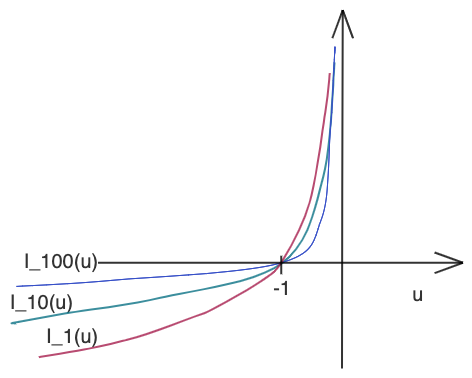
\includegraphics[scale=0.45]{images/ind_pic.png}
        \label{}
        \caption{$I_{\tau}(u)$функции.}
        \endminipage\hfill
        \minipage{0.45\textwidth}
        \centering
        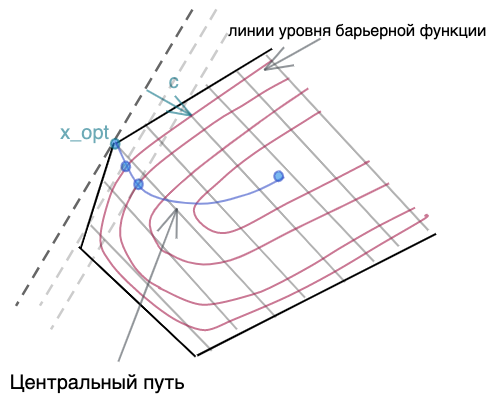
\includegraphics[scale=0.45]{images/path_pic.png}
        \label{}
        \caption{Центральный путь для примера.}
        \endminipage\hfill
\end{figure}



$L_{\tau}(x, \mu) = f(x) - \dfrac{1}{\tau} \sum_{i=1}^m log(-g_i(x)) + \mu^T(Ax - b)$

$\nabla_x L_{\tau}(\hat{x}, \hat{\mu}) = \nabla_x f(\hat{x}) + \dfrac{1}{\tau} \sum_{i=1}^m \dfrac{-\nabla_x g_i(\hat{x})}{g_i(\hat{x})} + A^T\hat{\mu} = 0$

При этом для исходной задачи:

$L_{\tau}(x, \mu, \lambda) = f(x) + \sum_{i=1}^m \lambda_i g_i(x) + \mu^T(Ax - b)$

$\nabla_x L_{\tau}(\hat{x}, \hat{\mu}, \hat{\lambda }) = \nabla_x f(\hat{x}) +
 \sum_{i=1}^m \nabla_x \hat{\lambda_i}g_i(\hat{x}) + A^T\hat{\mu} = 0$

 Тогда введем обозначение: $\hat{\lambda_i} = \dfrac{-1}{\tau g_i(\hat{x})}$


 Для $(\hat{x}(\tau), \hat{\mu}(\tau), \hat{\lambda}(\tau)):$

 \[
 \begin{cases}
 \nabla_x  L_{\tau}(\hat{x}, \hat{\mu}, \hat{\lambda }) = 0 \\
 A\hat{x} = b \\
\hat{ \lambda_i}  > 0 \ \forall i=1, \dots, m \\
\hat{\lambda_i} g_i(\hat{x}) = -\dfrac{1}{\tau} \ \forall i=1, \dots, m
\end{cases}
 \]


При $\tau \to + \infty$ $(\hat{x}(\tau), \hat{\mu}(\tau), \hat{\lambda}(\tau))$ удовлетворяет ККТ для исходной задачи

Введем двойственную функцию:

$g(\lambda, \mu) = inf_x L(x, \mu, \lambda)$

$g(\lambda, \mu) \leqslant f_{opt} \ \forall \mu, \forall \lambda > 0$

$g(\hat{\lambda}, \hat{\mu}) = L(\hat{x}, \hat{\mu}, \hat{\lambda}) \leqslant f_{opt}$

$f(\hat{x}) - f_{opt} \leqslant f(\hat{x}) - L(\hat{x}, \hat{\mu}, \hat{\lambda}) = f(\hat{x}) - f(\hat{x}) + \sum_{i=1}^m \hat{\lambda_i} g_i(\hat{x}) + \hat{\mu}^T(A\hat{x} - b)  = \dfrac{m}{\tau}$

$ \ (\hat{x} \text{ допустимое } \implies A\hat{x} = b)$

$\dfrac{m}{\tau} = \varepsilon, \ \tau = \dfrac{\varepsilon}{m}$

На практике постепенно увеличиваем $\tau$

\bigskip

Приведем общую схему метода:

\begin{algorithm}[H]
	\begin{algorithmic}[1]
		\Procedure{$logarithmic barrier$}{$x_0 \in D, Ax_0 = b, g_i(x_0) < 0 \ \forall i, \varepsilon, \tau_0, \nu > 1$}
		\For{$k=0, 1, 2, ...$}
		\State найти $\hat{x}(\tau_k)$ решение задачи
		$$ \begin{cases} f(x) - \dfrac{1}{\tau_k}\sum_i log(-g_i(x)) \to min_x \\ Ax=b \end{cases}$$
		с помощью метода Ньютона из начального приближения $x_k$
		\State $x_{k+1} \gets \hat{x}(\tau_k)$
		\If{$\dfrac{m}{\tau_k} \leqslant \varepsilon$} \textbf{break}
		\EndIf
		\State $\tau_{k+1} \gets min\left(\dfrac{m}{\varepsilon}, \tau_k \cdot \nu \right)$
		\EndFor
		\State \Return $\alpha_k$
		\EndProcedure
	\end{algorithmic}
\end{algorithm}

$\nu$ отвечает за трейдоф внешних и внутренних итераций: чем больше $\nu$, тем быстрее дойдем то $\tau_k = \dfrac{m}{\varepsilon}$, тем меньше будет внешних итераций, но тем хуже будет стартовая точка $x_k$, то есть тем больше внутренних итераций.

В качестве $x_0$ необходимо подать внутреннюю точку, иногда ее поиск довольно сложный, тогда нужно воспользоваться методом первой фазы (как в симплекс-методе)
